% This example is meant to be compiled with lualatex or xelatex
% The theme itself also supports pdflatex
\PassOptionsToPackage{unicode}{hyperref}
\documentclass[aspectratio=1610, 9pt]{beamer}

% Load packages you need here
\usepackage{polyglossia}
\setmainlanguage{german}

\usepackage{csquotes}


\usepackage{amsmath}
\usepackage{amssymb}
\usepackage{mathtools}

\usepackage{hyperref}
\usepackage{bookmark}

\usepackage{algorithm2e}

% load the theme after all packages

\usetheme[
  showtotalframes, % show total number of frames in the footline
]{tudo}

% Put settings here, like
\unimathsetup{
  math-style=ISO,
  bold-style=ISO,
  nabla=upright,
  partial=upright,
  mathrm=sym,
}

\title{Ist das Universum ein Computer?}
\author[J.~Speer]{Jannis Speer}
\date{17.12.20}
\institute{Big Questions Seminar}
\titlegraphic{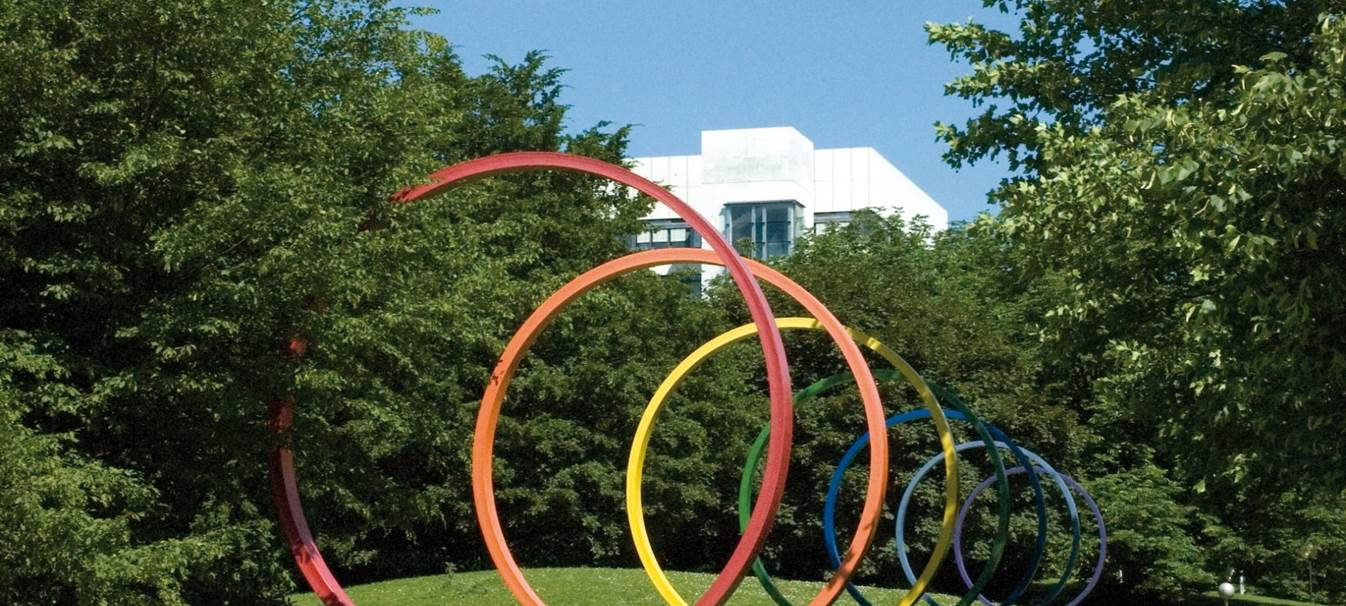
\includegraphics[width=0.7\textwidth]{images/tudo-title-2.jpg}}


\begin{document}

\maketitle

\begin{frame}{Inhalt}
  \begin{itemize}
    \item
  \end{itemize}
\end{frame}

%\begin{frame}{Inhalt}
%  \tableofcontents
%\end{frame}

\begin{frame}{Historische Einführung: Digitale Physik}
  \begin{itemize}
    \item ursprüngliche Idee: Konrad Zuses Buch Rechnender Raum (1969)
    \item Hypothese: Universum ist digitaler Computer, genauer: zellulärer Automat
    \item Komatibilität von Computern mit: \\Informationstheorie, statistischer Mechanik, Quantenmechanik
    \item Begriff geprägt durch  Edward Fredkin, alternativ: digitale Philosophie
    \item[]
    \item[\rightarrow] Digitale Physik: Theorien mit Prämise, Universum durch Information beschreibbar ist
  \end{itemize}
\end{frame}

\begin{frame}{Digitale Physik - verschiedene Perspektiven}
  \begin{itemize}
    \item Weizsäckers Quantentheorie der Ur-Alternativen:
      \begin{itemize}
        \item[\bullet] lediglich 2  Entitäten: Struktur der Zeit, binäre Alternativen
        \item[\bullet] abstrakt, nicht-lokal, keine feldtheoretischen Voraussetzungen
      \end{itemize}
    \item[]
    \item Wheelers It from Bit:
      \begin{itemize}
        \item[\bullet] klassisch: Realität existiert und wird gemessen
        \item[\bullet] hier: Messung schafft Realität
      \end{itemize}
    \item[]
    \item Pancomputationalism:
      \begin{itemize}
        \item[\bullet] Digitaler Computer vs. Quantencomputer
        \item[\bullet] Zufälligkeit und Komplexität des Universums? Effizienz?
      \end{itemize}
    \item[]
    \item Tegmarks Mathematical-Universe-Hypothese (MUH)
      \begin{itemize}
        \item[\bullet] Universum ist Mathematik, mathematische Existenz = physikalische Existenz
      \end{itemize}
  \end{itemize}
\end{frame}

\begin{frame}{Informationstheorie}
  \begin{figure}
    \begin{minipage}{0.7\textwidth}
      \begin{itemize}
        \item[] ... beschäftigt sich mit Quantifizierung, Speicherung und Übertragung von Information
        \item[]
        \item Konzept von Information hat verschiedene Bedeutungen \\verwandt mit: Nachricht, Kommunikation, Daten, Wissen
        \item hier: Information ist Folge von Symbolen aus einem Alphabet $Z = \{z_1, z_2,...,z_m\}$
        \item Informationsgehalt eines Zeichens: $I(z) = -\log_a(p_z)$ \\mit Wahrscheinlichkeit $p_z$, Mächtigkeit $a$
        \item Entropie eines Zeichens (Shannon): $H = E[I] = \sum_{z \in Z}{p_z I(z)} = - \sum_{z \in Z}{ p_z \log_a(p_z)}$
      \end{itemize}
    \end{minipage}
    \hfill
    \begin{minipage}{0.28\textwidth}
      \begin{figure}
        \includegraphics[width=0.8\textwidth]{images/binär.jpg}
        \caption{binäre Information}
      \end{figure}
    \end{minipage}
  \end{figure}
\end{frame}

\begin{frame}{physikalische Information und Entropie}
  \begin{itemize}
    \item Information beschreibt physikalisches System:
    \begin{itemize}
      \item[\bullet] Information löst Ungewissheit über Zustand eines physikalischen Systems
      \item[\bullet] Information ist Messung für Wahrscheinlichkeit eines Zustandes
    \end{itemize}
    \item[]
    \item $\text{fehlende Information} = \text{nötige Information, um Zustand zu beschreiben} = I = -k \sum_{i=1}^n{p_i \ln(p_i)}$ \\ mit $p_i$ der Wahrscheinlichkeiten der $n$ Zustände des Systems
    \item[]
    \begin{itemize}
      \item[\rightarrow] binäre Entropie der Informationstheorie: $k = \ln(2)^{-1}$
      \item[\rightarrow] Gibbs Entropie: $k = k_b$
    \end{itemize}
    \item Von Neumann Entropie, QM-Analogon: $S(\rho) = -Tr(\rho \ln\rho)$ mit Dichtematrix $\rho$
  \end{itemize}
\end{frame}

\begin{frame}{Algorithmische Informationstheorie}
  \begin{itemize}
    \item Bestimmung des Informationsgehalt über Kolmogorow-Komplexität
    \item Kolmogorow-Komplexität:
    \begin{itemize}
      \item Informationsgehalts einer Zeichenkette = Länge des kleinsten Algorithmus, der Zeichenkette erzeugt
      \item nicht berechenbar, aufgrund des Halteproblems kleinster Algorithmus nicht bestimmbar
      \item unabhängig von der verwendeten universellen Programmiersprache abgesehen von additiver Konstante $c$
    \end{itemize}
  \end{itemize}
  \begin{figure}
    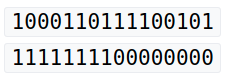
\includegraphics[width=0.2\textwidth]{images/kolmo.png}
    %\caption{binäre Information}
  \end{figure}
  \begin{itemize}
    \item algorithmic randomness:
    \begin{itemize}
      \item Zeichenkette ist zufällig, wenn Kolmogorow-Komplexität $>=$ Länge der Zecihenkette
      \item Zufälligkeit einer endlichen Zeichenkette abhängig von universellen Programmiersprache
      %\item Löf randomness: unendliche Folge $S$ ist $c$-inkompressibel, wenn Teilfoge $w$
    \end{itemize}
  \end{itemize}
\end{frame}

\begin{frame}{Digitale Information, Boolesche Algebra, Klassische Logik}
  \begin{figure}
    \begin{minipage}{0.7\textwidth}
      \begin{itemize}
        \item Digitale Information: diskrete endliche Darstellung \rightarrow Ziffern, Buchstaben \rightarrow binär
        \item Boolesche Algebra mit Operatoren:
        \item[] $\land$ UND $\lor$ ODER $\lnot$ NICHT
        \item klassische Logik:
        \begin{itemize}
          \item Prinzip der Zweiwertigkeit
          \item Prinzip der Extensionalität
        \end{itemize}
      \end{itemize}
    \end{minipage}
    \hfill
    \begin{minipage}{0.28\textwidth}
      \begin{figure}
        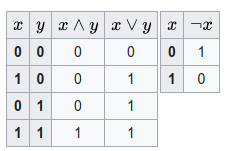
\includegraphics[width=0.8\textwidth]{images/bool.png}
        \caption{Boolesche Algebra.}
      \end{figure}
    \end{minipage}
  \end{figure}
\end{frame}

\begin{frame}{Vor Turing}
  \begin{itemize}
    \item Formulierung des Hilbertprogramms in 1920er
    \item Ziel: Nachweis der Widerspruchsfreiheit der Axiomensysteme der Mathematik
    \item[\rightarrow] Entscheidungsproblem: \enquote{First, was mathematics complete ... Second, was mathematics consistent ... \\ And thirdly, was mathematics decidable?}
    \item[\rightarrow] Beantwortung durch Gödels Unvollständigkeitssätze
    \item[]
    \item Was ist ein Algorithmus?
  \end{itemize}

\end{frame}

\begin{frame}{Turingmaschine - informelle Einführung}
  \begin{figure}
    \begin{minipage}{0.49\textwidth}
      \begin{itemize}
        \item Interpretation von Logik als Prozess
        \item Definition Algorithmus und der Berechenbarkeit
        \item Analogie eines denkenden, lesenden und schreibenden Mathematikers
      \end{itemize}
      \begin{figure}
        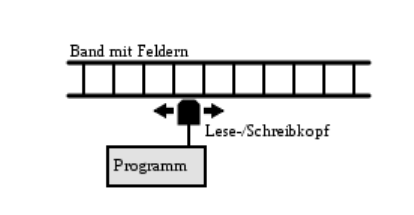
\includegraphics[width=0.8\textwidth]{images/turing.png}
        \caption{Turingmaschine.}
      \end{figure}
    \end{minipage}
    \hfill
    \begin{minipage}{0.49\textwidth}
      \begin{itemize}
        \item Turingmaschine:
        \begin{itemize}
          \item Speicherband: unendlich viele, sequentiell angeordnete Felder
          \item Feld: nimmt einen von endlich vielen Zuständen an
          \item Lese-Schreib-Kopf: Verarbeitung von Information, nimmt einen von endlich vielen Zuständen an
        \end{itemize}
        \item Prozess:
        \begin{itemize}
          \item Kopf liest Zustand des aktuellen Feldes
          \item Kopf verarbeitet eignen Zustand und Feldzustand \\ (Überführungsfunktion)
          \item Änderung des Kopf und Feldzustandes
          \item Kopf bewegt sich ein Feld nach rechts oder links
        \end{itemize}
      \end{itemize}
    \end{minipage}
  \end{figure}
\end{frame}

\begin{frame}{Anmerkungen zur Turingmaschine}
  \begin{figure}
    \begin{minipage}{0.29\textwidth}
      Algorithmus:
      \begin{itemize}
        \item Ausfürbarkeit
        \item Statistische Finitheit
        \item Dynamische Finitheit
        \item Terminierung
        \item optional:
        \begin{itemize}
          \item[\bullet] Determiniertheit
          \item[\bullet] Determinismus
        \end{itemize}
      \end{itemize}
    \end{minipage}
    \hfill
    \begin{minipage}{0.69\textwidth}
      Universelle Turingmaschine (UTM):
      \begin{itemize}
        \item UTM simuliert beliebig Turingmaschine für beliebigen Input
        \item Speicherung der Turingmaschine und des Inputs auf Speicherband der UTM
        \item[\rightarrow] Halteproblem
      \end{itemize}
      \begin{figure}
        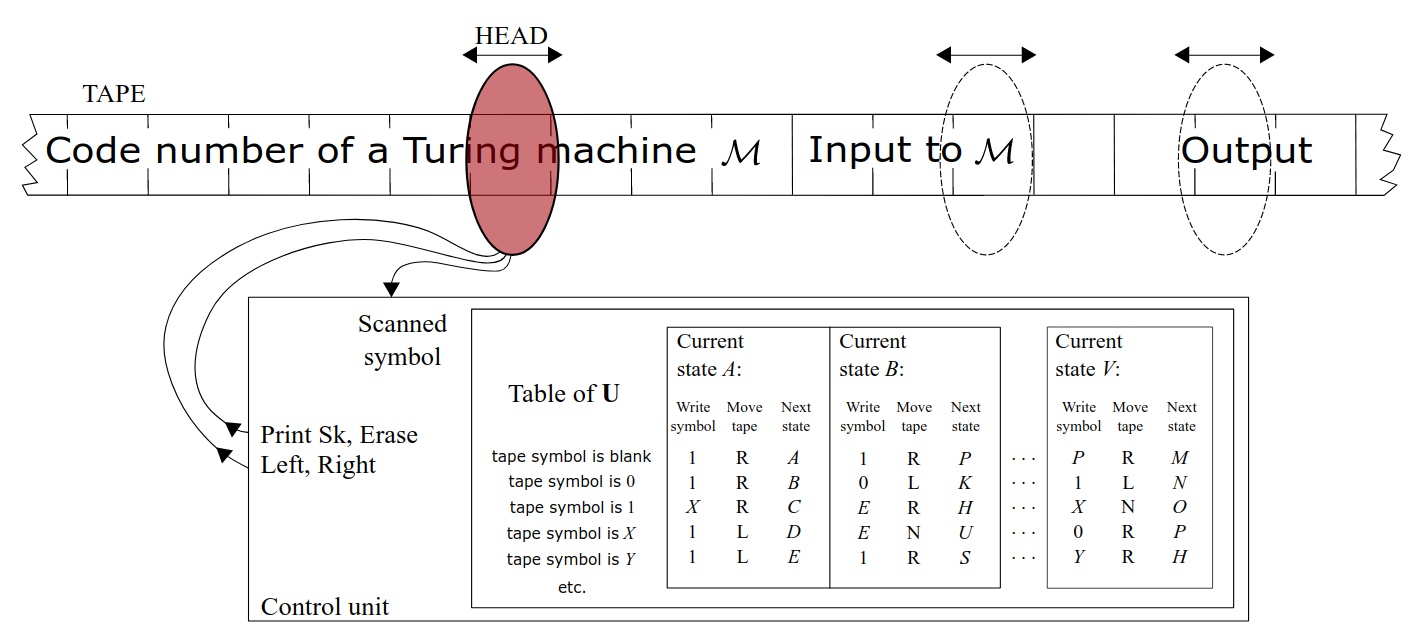
\includegraphics[width=0.8\textwidth]{images/UTM.png}
        \caption{Turingmaschine.}
      \end{figure}
    \end{minipage}
  \end{figure}
\end{frame}

\begin{frame}{Anmerkungen zur Turingmaschine}
  \begin{figure}
    \begin{minipage}{0.49\textwidth}
      Halteproblem:
      \begin{itemize}
        \item Analog zu Gödels Unvollständigkeitssatz:
        \begin{itemize}
          \item Logik ist selbst-widersprechend und unvollständig
          \item Problem von auf sich selbst bezogene Behauptungen
          \item Lügner-Paradox: \enquote{Dieser Satz ist falsch.}
        \end{itemize}
        \item Keine UTM kann Frage beantworten, ob eine beliebige Turingmaschine anhält (Antwort liefert)
        \item Konstruktion von selbst-widersprechender UTM:
      \end{itemize}
      \begin{algorithm}[H]
        \KwResult{Hält beliebige Turingmaschine T nicht an?}
        \Begin{
          T = beliebige Turingmaschine \;
          Bestimme ob T anhält \;
            \If{T hält nicht an == True}{return Antwort\;}
        }
      \end{algorithm}
    \end{minipage}
    \hfill
    \begin{minipage}{0.49\textwidth}
      Church-Turing-These:
      \begin{itemize}
        \item Jede intuitiv berechenbare Funktion kann durch eine UTM berechnet werden
        \item intuitiv berechenbar: mathematisch ungenauer Begriff
        \item Turing-berechenbar: Existenz von (terminierendem) Algorithmus
        \item[]
        \item striktere, physikalische Version: Church–Turing–Deutsch-Hypothese
        \item[] UTM kann jeden phyiskalischen Porzess simulieren
      \end{itemize}
    \end{minipage}
  \end{figure}
\end{frame}


\begin{frame}{Universum als digitaler Computer}

\end{frame}

\begin{frame}{Universum als digitaler Computer 2}

\end{frame}

\begin{frame}{Effizienz von digitalen Computern}

\end{frame}

\begin{frame}{Quantencomputer}

\end{frame}

\begin{frame}{Quantencomputer 2}

\end{frame}

\begin{frame}{Universum als Quantencomputer}

\end{frame}

\begin{frame}{Universum als Quantencomputer 2}

\end{frame}

\begin{frame}{Digitaler Computer vs. Quantencomputer}

\end{frame}

\begin{frame}{Gegenposition - Das Universum ist kein Computer}

\end{frame}

\begin{frame}{Ausblick}

\end{frame}

\end{document}
